\chapter{Chasse aux traitres (traitor tracing)}
    \section{Système DVB (Digital Video Broadcasting)}
        \subsection{Description}
        \begin{figure}[H]
            \centering
            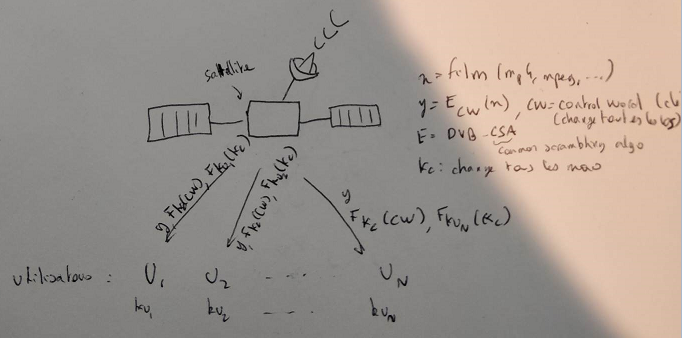
\includegraphics[width=.5\textwidth]{pictures/2_3}
        \end{figure} \noindent
        \begin{figure}[H]
            \centering
            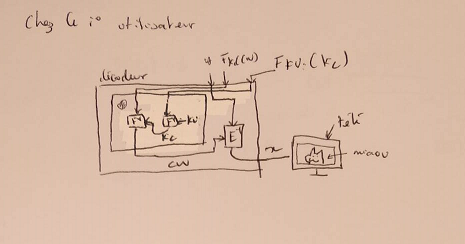
\includegraphics[width=.5\textwidth]{pictures/2_4}
        \end{figure} \noindent
        \subsection{Attaques possibles}
            \begin{description}
                \item[Idée 1 :] Rediffuser $x$ (en direct ou en différé). Non traçable. Contres-mesures
                \begin{itemize}
                    \item Téléviseur sécurisé
                    \item Watermarking : ajouter dans un contenu une information secrète indétectable, qui résiste à des tentatives de l'effacer, pour savoir quel utilisateur a diffusé $x$ (lié à la stéganographie).
                \end{itemize}
                \item[Idée 2 :] rediffuser CW. Non traçable. On peut mettre $E^{-1}$ du décodeur dans une carte à puce pour que CW soit difficile d'accès. 
                \item[Idée 3 :] Diffuser KC. Non traçable. Comme KC n'apparaît que dans une carte à puce, ils faut prendre des mesures pour les attaques DPA.
                \item[Idée 4 :] Envoyer K$U_i$ (trouvée par exemple par DPA). Traçable
                \begin{itemize}
                    \item En boîte blanche : il récupère K$U_i$ et retrouve à qui appartient la clé
                    \item En boîte noire :
                    \begin{figure}[H]
                        \centering
                        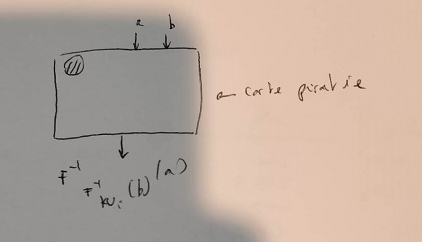
\includegraphics[width=.5\textwidth]{pictures/2_5}
                    \end{figure} \noindent
                    L'opérateur cherche K$U_i$, mais ne cherche pas dans tout l'espace des clés possibles, mais que dans les clés distribuées aux utilisateurs, donc il retrouve facilement K$U_i$ par recherche exhaustive. 
                \end{itemize}
                De plus, des contres-mesures anti DPA rendent difficile l'accès à K$U_i$.
            \end{description}

    \section{Broadcast encryption et traitor tracing}
        \subsection{Problématique}
            Envoyer un contenu $x$ à $N$ utilisateurs.
            \subsubsection{Solution 1}
                \begin{figure}[H]
                    \centering
                    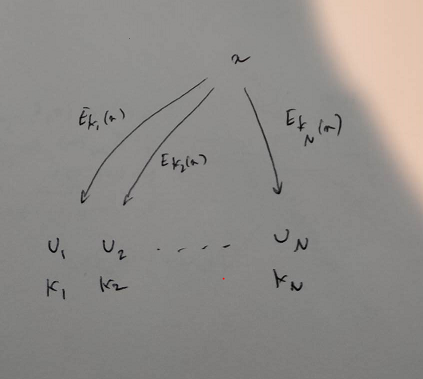
\includegraphics[width=.5\textwidth]{pictures/2_6}
                \end{figure} \noindent
                \begin{itemize}
                    \item Taille des données à diffuser : $N \times \card{x}$.
                    \item Résiste à des collusions de $N$ utilisateurs.
                \end{itemize}

            \subsubsection{Solution 2}
                \begin{figure}[H]
                    \centering
                    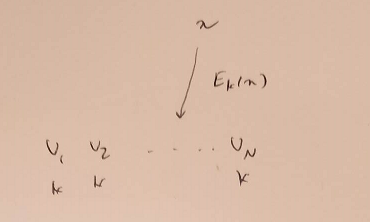
\includegraphics[width=.5\textwidth]{pictures/2_7}
                \end{figure} \noindent
                \begin{itemize}
                    \item Taille des données : $1 \times \card{x}$.
                    \item Résiste à aucune collusion.
                \end{itemize}

        \subsection{Protocole de Chor-Fiat-Naor (1994)}
            On écrit $x = x_1 \oplus x_2 \oplus \cdots \oplus x_t$. On génère des clés $K_{1, 0}, K_{2, 0}, \cdots, K_{t, 0}$, et $K_{1, 1}, K_{2, 1}, \cdots, K_{t, 1}$. On donne à chaque utilisateur une clé de la forme $(K_{1, \varepsilon_1}, K_{2, \varepsilon_2}, \cdots, K_{t, \varepsilon_t})$, où $\varepsilon_i \in \{0, 1\}$. On diffuse $E_{K_{i, 0}}(x_i)$ et $E_{K_{i, 1}}(x_i)$. L'utilisateur à de quoi déchiffrer chaque bout de $x$, et le reconstituer en xorant.
            \begin{itemize}
                \item Taille des données : $2t\card{x}$, $2^t \geq N$, donc $t \simeq \log_2(N)$.
                \item Résiste à des collusions de $1$ utilisateurs.
            \end{itemize}

        \subsection{Utilisation de codes correcteurs}
            \begin{defi}
                Un colde linéaire binaire (code) de longeur $n$ est une partie $C$ de $\mathbb{F}_2^n$ stable par addition (i.e. un sous espace vectoriel de $\mathbb{F}_2^n$). Un vecteur de $C$ est appelé mot de $C$. Le support de $x \in \mathbb{F}_2^n$ est 
                \begin{align*}
                    \mathrm{supp} (x) = \{i \in \lcc 1, n \rcc \mid x_i \neq 0\}
                \end{align*}
                Le poids de $x$ est $\card{x} = \card{\mathrm{supp} (x)}$ (poids de Hamming). La distance de Hamming entre deux vecteurs $x, y \in \mathbb{F}_2^n$ est 
                \begin{align*}
                    d(x, y) = \card{x - y}
                \end{align*}
                La distance minimale du code $C$ est
                \begin{align*}
                    d(C) = \min_{x \in C,\, x \neq 0} \card{x}
                \end{align*}
            \end{defi}

            \begin{description}
                \item[Problème du codage :] 
                \begin{itemize}
                    \item On veut transmettre $m$ sous forme d'un vecteur $x$.
                    \item Canal de communication imparfait \cor{Figure 8}
                \end{itemize}
                \item[Décodage :] Bob prend parmi les mots de $C$ celui qui est le plus proche de $v$ pour la distance de hamming.
            \end{description}
            \begin{theo}
                Si un code $C$ a une distance minimale $d$ et si le nombre d'erreurs est $\leq \frac{d - 1}2$, alors le décodage permet toujours de retrouver $x$ à partir de $v = x + e$
            \end{theo}
            \begin{proof}
                Montrons que $x$ est le mot de $C$ le plus proche de $v$. Soit $y \in C$, $y \neq x$, alors il suffit de montrer que $d(y, v) > d(x, v)$. Mais $d(x, y) \leq d(x, v) + d(v, y)$, soit 
                \begin{align*}
                    d(v, y) \geq d(x, y) - e \geq d - \frac{d - 1}2 = \frac{d + 1}2 > d(x, v)
                \end{align*}
            \end{proof}
                